% Number 920
% CAPMG  Units 
% Rocket upwards - max. v, h?
% JG

% Watermark
\AddToShipoutPicture*{\BackgroundPic}

\addtocounter {ProbNum} {1}

%\begin{floatingfigure}[r]{.44\textwidth}
%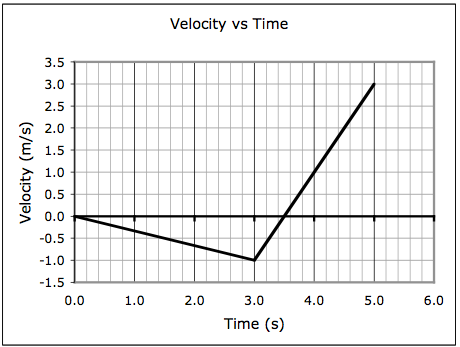
\includegraphics[scale=.54]{/Users/jgates/desktop/latex/pics/vgraph6}
%\end{floatingfigure}
 
{\bf \Large{\arabic{ProbNum}}} A rocket launches and travels upwards with an acceleration of ${4.5~\tfrac{m}{s^2}}$ for 6 seconds; at that point it runs out of fuel and goes into freefall.   \bigskip

Determine the rocket's maximum speed on the upwards trip and maximum height using graphical methods.  \vfill


%\begin{center}
%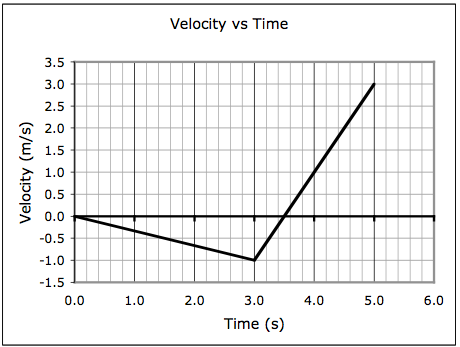
\includegraphics[scale=1]{/Users/jgates/desktop/latex/pics/vgraph6}
%\end{center}


\newpage